\noindent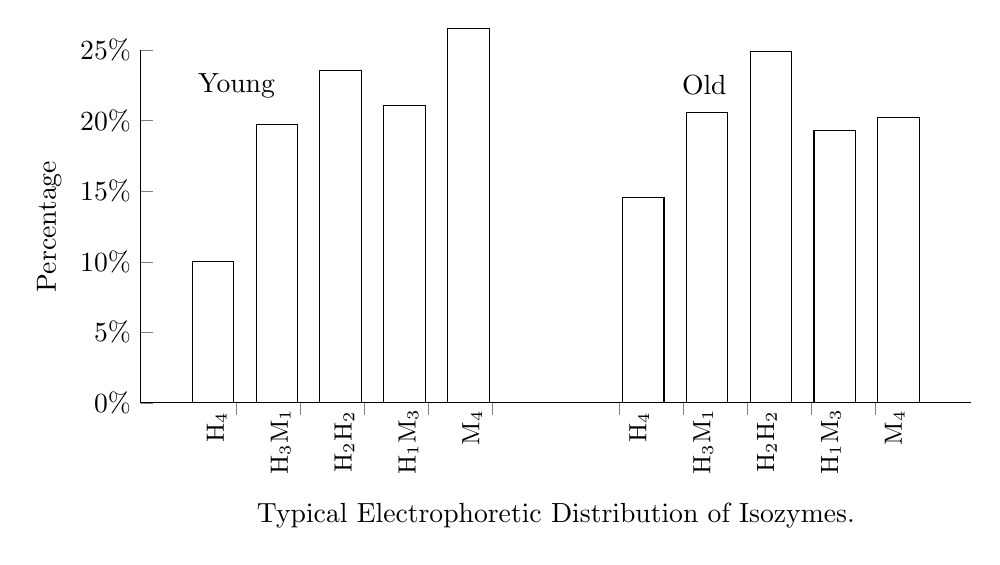
\begin{tikzpicture}
\begin{axis}[
    ybar,
    bar width=15pt,
    enlarge x limits=0.15,
    ylabel={Percentage},
    xlabel={Typical Electrophoretic Distribution of Isozymes.},
    ytick={0,5,10,15,20,25},
    yticklabels={0\%,5\%,10\%,15\%,20\%,25\%},
    ymin=0,
    ymax=25,
    axis lines*=left,
    xtick={1,2,3,4,5,7,8,9,10,11},
    xticklabels={,,,,,,,,,,}, 
    x tick label style={font=\small},
    width=\linewidth,
    height=0.5\linewidth,
    legend style={draw=none},
    clip=false,
    xlabel style={yshift=-5ex}
]

\addplot[fill=white, draw=black] coordinates {
    (1,10.042735042735043)  
    (2,19.71153846153846)  
    (3,23.55769230769231)   
    (4,21.04700854700855)  
    (5,26.549145299145305)   
};

\addplot[fill=white, draw=black] coordinates {
    (7,14.529914529914532)  
    (8,20.566239316239322)  
    (9,24.893162393162395)  
    (10,19.284188034188038) 
    (11,20.219017094017094)  
};

\node[rotate=90, anchor=south] at (axis cs:1,-1.75) {\small $\mathrm{H}_4$};
\node[rotate=90, anchor=south] at (axis cs:2,-2.75) {\small $\mathrm{H}_3\mathrm{M}_1$};
\node[rotate=90, anchor=south] at (axis cs:3,-2.75) {\small $\mathrm{H}_2\mathrm{H}_2$};
\node[rotate=90, anchor=south] at (axis cs:4,-2.75) {\small $\mathrm{H}_1\mathrm{M}_3$};
\node[rotate=90, anchor=south] at (axis cs:5,-1.75) {\small $\mathrm{M}_4$};

\node[rotate=90, anchor=north] at (axis cs:7,-1.75) {\small $\mathrm{H}_4$};
\node[rotate=90, anchor=north] at (axis cs:8,-2.75) {\small $\mathrm{H}_3\mathrm{M}_1$};
\node[rotate=90, anchor=north] at (axis cs:9,-2.75) {\small $\mathrm{H}_2\mathrm{H}_2$};
\node[rotate=90, anchor=north] at (axis cs:10,-2.75) {\small $\mathrm{H}_1\mathrm{M}_3$};
\node[rotate=90, anchor=north] at (axis cs:11,-1.75) {\small $\mathrm{M}_4$};

\node at (axis cs:1,22.5) {Young};
\node at (axis cs:8.325,22.5) {Old};

\end{axis}
\end{tikzpicture}